\section{Ottimizzazione DB}

\subsection{Indici}

Un \textbf{indice} in un sistema di gestione di database (DBMS) è una struttura dati organizzata che consente di individuare rapidamente un determinato record all'interno di un file di dati. Uno dei principali vantaggi dell'utilizzo degli indici è il miglioramento delle prestazioni delle query: gli indici permettono di ridurre il tempo necessario per cercare i dati, evitando una scansione completa della tabella.

Creare indici sui campi che vengono frequentemente utilizzati nei filtri delle query (ad esempio, con condizioni \texttt{WHERE}, \texttt{JOIN}, \texttt{ORDER BY} o \texttt{GROUP BY}) può velocizzare significativamente l'elaborazione delle richieste, ottimizzando il sistema nel suo complesso.

Tuttavia, è importante bilanciare l'uso degli indici per evitare costi aggiuntivi durante le operazioni di scrittura come \texttt{INSERT}, \texttt{UPDATE} e \texttt{DELETE}, poiché gli indici devono essere aggiornati ogni volta che i dati della tabella vengono modificati.

Tralasciando gli indici sulla chiave primaria, in quanto il DBMS crea un indice per ogni chiave primaria della tabella, abbiamo pensato di aggiungere questi indici: \\

\begin{lstlisting}
CREATE INDEX idx_missioni_stato ON MISSIONI(Stato); 
-- utile per filtrare missioni sullo stato

CREATE INDEX idx_membri_ruolo ON MEMBRI(Ruolo); 
-- utile per filtrare sul ruolo dei membri

CREATE INDEX idx_robot_tipo ON ROBOT(Tipo); 
-- utile per filtrare sul tipo di robot

CREATE INDEX idx_report_data ON REPORT(Data);

CREATE INDEX idx_rilevazioni_sensori_data ON RILEVAZIONI(Sensori, Data);
\end{lstlisting}

\subsection{Concorrenza}

Per la gestione della concorrenza abbiamo scelto di adottare il protocollo \textbf{2PL stretto}, una variante del \textbf{2PL}. Entrambi i protocolli si basano sul meccanismo del \textbf{lock}, che consente di gestire la concorrenza e garantire la \textbf{serializzabilità delle transazioni}.

Il suo funzionamento prevede:

\begin{itemize}
    \item \texttt{lock()}: ogni oggetto è protetto da un lock;
    \item \texttt{read\_lock()}: se una transazione vuole effettuare una lettura su uno oggetto. Più transazioni possono leggere contemporaneamente lo stesso oggetto (condivisione).
    \item \texttt{write\_lock()}: è esclusivo e consente a una sola transazione di modificare l'oggetto per volta.
    \item \texttt{unlock()}: Ogni lock, una volta terminata l'operazione, deve essere rilasciato (unlock).
\end{itemize}

Gli oggetti possono trovarsi in tre stati: \textbf{libero}, \textbf{bloccato in lettura}, o \textbf{bloccato in scrittura}.

La scelta del \textbf{2PL stretto} rispetto al \textbf{2PL} è dovuta al fatto che il \textbf{2PL stretto} evita l'anomalia delle \textbf{letture sporche} (dirty reads), che possono verificarsi in altri approcci di gestione della concorrenza.

Il 2PL stretto prevede due fasi:

\begin{itemize}
    \item \textbf{fase crescente}: è la fase in cui una transazione acquisisce mediante \texttt{read\_lock} e \texttt{write\_lock} tutte le risorse su cui dovrà effettuare operazioni di lettura e scrittura.
    \item \textbf{fase decrescente}: è la fase in cui attraverso l'\texttt{unlock} si vanno a rilasciare le risorse. In particolare questa fase nel caso di 2PL stretto può essere effettuata solo se la transazione termina con una commit o con un abort.
\end{itemize}

Questo approccio garantisce che le transazioni siano serializzabili, impedendo conflitti e mantenendo la consistenza dei dati.

\subsection{Affidabilità}

Il controllo di \textbf{affidabilità} in un sistema di basi di dati ha come obiettivo principale il \textbf{ripristino} dello stato corretto del sistema (recovery) in seguito a guasti accidentali o intenzionali, che possano compromettere la funzionalità del sistema stesso. I guasti possono essere legati sia a malfunzionamenti hardware (ad esempio, guasti su disco o memoria) che software (ad esempio, crash di applicazioni o errori di sistema).

Il sistema di affidabilità si basa sulla gestione delle \textbf{transazioni}, che sono le unità fondamentali delle operazioni nel database, garantendo \textbf{atomicità} (le transazioni sono eseguite in modo completo o non eseguite affatto) e \textbf{persistenza} (i dati delle transazioni devono essere memorizzati in modo permanente una volta che la transazione è stata completata correttamente).

\subsubsection{Backup}

Per garantire un alto livello di affidabilità, il nostro sistema di database implementa la strategia di backup RAID 1, che offre una soluzione di mirroring. In un sistema RAID 1, ogni dato scritto sul disco primario viene duplicato in tempo reale su un disco secondario, chiamato "mirror". Questa tecnica garantisce che, in caso di guasto di uno dei dischi, i dati siano ancora disponibili sull'altro disco, riducendo il rischio di perdita di informazioni e migliorando la disponibilità del sistema.

\begin{figure}[h]
    \centering
    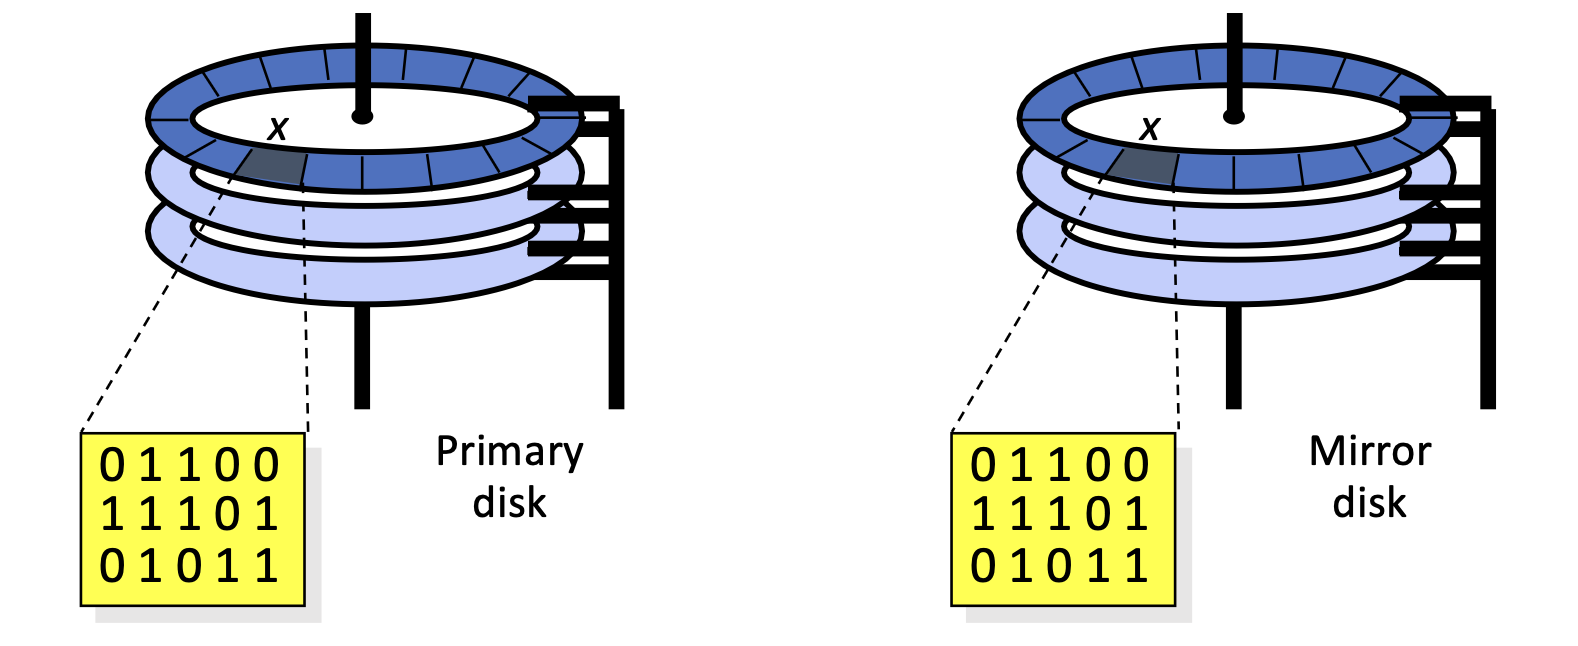
\includegraphics[width=0.5\textwidth]{Media/raid.png}
    \caption{RAID 1 Mirroring}
    \label{fig:raid}
\end{figure}

\subsubsection{Recovery}

Il gestore dell’affidabilità deve gestire l’esecuzione dei comandi transazionali di \texttt{begin transaction}, \texttt{commit}, \texttt{rollback} e tutte le operazioni di ripristino dopo i guasti.

Per poter effettuare ciò, il gestore deve possedere un file di log: un file presente su memoria stabile che registra tutte le operazioni svolte dalle transazioni nel loro ordine di esecuzione.

Il log è quindi una sorta di “diario di bordo” che, in un qualsiasi istante, permette di ricostituire il contenuto corretto della base dei dati a seguito di malfunzionamenti.

\begin{figure}[h]
    \centering
    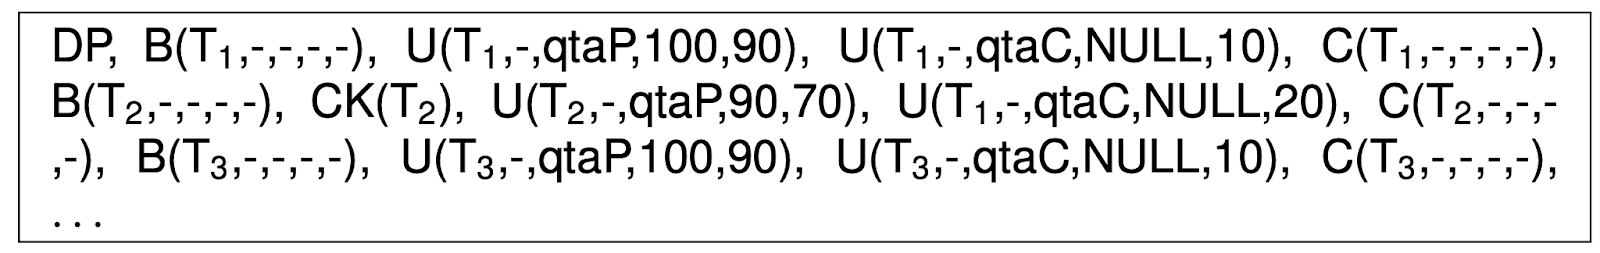
\includegraphics[width=0.5\textwidth]{Media/log.png}
    \caption{File di log}
    \label{fig:log}
\end{figure}

\paragraph{Tecniche di recovery}

\begin{itemize}
    \item \textbf{Ripresa a freddo}: Nel caso di guasti hard sui dispositivi di memoria di massa (es. guasti ai dischi rigidi) si perde sia la memoria centrale che quella secondaria, ma la memoria stabile (come i dispositivi di backup) rimane intatta. In queste situazioni, viene effettuata la ripresa a freddo (cold restart), che richiede un ripristino più approfondito, attingendo ai backup e ai log per recuperare i dati persi.
    \item \textbf{Ripresa a caldo}: Nel caso di guasti soft (es. errori di programma, crash di sistema, caduta di tensione, ecc.) si perde il contenuto della sola memoria centrale (mentre rimangono intatte la memoria secondaria e quella stabile). In tali situazioni, viene effettuata la cosiddetta ripresa a caldo (warm restart).
\end{itemize}

In entrambi i casi, la procedura di ripristino avviene nelle seguenti fasi (modello fail-stop):

\begin{enumerate}
    \item si forza l’arresto completo delle transazioni attive sul sistema di basi di dati;
    \item viene ripristinato il corretto funzionamento del sistema operativo;
    \item viene effettuata la procedura di ripristino.
\end{enumerate}
